%%
%%  chapter05.tex - Obstacle Detection and Planning for Autonomous Vehicles based on Computer Vision Techniques
%%
%%  Copyright 2014 Néstor Morales <nestor@isaatc.ull.es>
%%
%%  This work is licensed under a Creative Commons Attribution 4.0 International License.
%%

\graphicspath{{./images/chapter05/bmps/}{./images/chapter05/vects/}{./images/chapter05/}}

\chapter{3D object tracking}\label{ch:chapter05}

As we have seen in previous chapters, we still have not solved completely the problem of detection and tracking of the obstacles. Image comparison could be, as said, a good input point for an obstacle classifier, but it is still not able to locate obstacles in the real world with respect to a map o to the vehicle. Also, it is not able to track the obstacles and it is very dependent on the goodness of the database of the area in which the vehicle is driving. Non-rigid point set registration method is not able to detect obstacles using moving cameras. \notsure{Stixels can be a solution, but they do not consider obstacles further from a first plane and they assume a flat road}. 

In this chapter, we will describe a method that, using a point cloud generated from a pair of moving stereo cameras, is able to detect obstacles and model them as a set of voxels. Also, it is able to decide the direction in which objects are moving to. The method described here is inspired in the work by \cite{danescu2012particle}, in the way that a particle filter is used over an occupancy grid in order to detect the obstacles and their directions. However, this method uses a two-dimensional grid. As said in section \ref{ch:chapter01_02_05}, methods based on such a grid are related to which we named as 2.5D methods. The main disadvantages of this kind of methods is that they consider all the obstacles as lying in the ground, and are represented as a convex cuboid that doesn't take into account the complexities of certain obstacles.
As commented in previous sections, Verdino is thought to work in crowded areas, like pedestrian streets or touristic complexes, in which an overestimation of the size of obstacles can lead to an inefficient behavior. So we decided to extend the original method of \cite{danescu2012particle} in order to make it fully three-dimensional, by using a voxelized grid instead of the original cartesian/polar grid, and including some improvements in order to reduce the number of fake positives, among others.

\section{The Method}\label{ch:chapter05_01}

In this method, we generate a voxelized occupancy grid in which the world surrounding the vehicle is divided into a discrete number of voxels of the same size. For each voxel, a occupancy probability is assigned based on the number of points inside the volume represented by it and its neighborhood. Also, during the process, a set of particles will be assigned dynamically during the execution, based on a 3D generalization of the weighting and resampling mechanism described in \cite{isard1998condensation}. These particles will have a double function:
\begin{enumerate}
 \item Denoting hypotheses (as happens with classical particle filters).
 \item Being the building blocks of our world model.
\end{enumerate}

Like this, at each frame, the set of particles obtained in the previous frame (each of these with a certain pose ${(x, y, z)}$ and speed ${(vx, vy, vz)}$) will be evolved using their movement model and assigned to the corresponding voxel, attending to the time that passed between frames and the ego-motion. Then, these particles are re-weighted and resampled.

At this point, particles that passed the resampling process are used to construct the objects that model the environment, joining all these voxels that share a similar orientation and speed. This object reconstruction is done by using a flood fill approach, in a way quite similar to that described in \cite{broggi2013}, but using the vectors of each voxel, instead of color information, as done in their work.

This particle-based approach inherits some advantages from the previous work by \cite{danescu2012particle}:
\begin{itemize}
 \item \emph{It is not necessary to estimate the probability distribution of the speed or the orientation.} These distributions, which in the past have been approximated as histograms (\cite{chen2006dynamic}), Gaussian mixtures (\cite{gindele2009bayesian}) or higher dimensions (\cite{coue2006bayesian}), are not required anymore due to the use the particles. This distribution is obtained directly from the surviving particles of each voxel. 
 \item \emph{Easy encoding of the past and present knowledge from sensor data.} The usage of a voxel grid makes this easier, and allows updating it dynamically when new information is available with a little computational cost.
\end{itemize}

Also, we add some new advantages in our approach:
\begin{itemize}
 \item \emph{Hierarchical object pose, orientation and speed detection.} Object units are detected at lower level as individual voxels, for which we know their individual speed and pose. Joining all these voxels together, we obtain the whole obstacle, whose pose and speed is directly dependent on the voxels which compose it. 
 \item \emph{Fully 3D perception of the object detected.} No previous assumption of the shape of the obstacles is taken, providing an accurate estimation of complex obstacles. The usage of voxels instead of cuboids, allows to have a clear idea of the actual shape of an obstacle, avoiding the overestimation of their real size, which is not acceptable for an application like that described in this Thesis. In this sense, we can have an accurate idea of 3D boundaries of an obstacle or reject it in case it is hanging, like in the case of traffic lights.
 \item \emph{No color information is used.} As we do not use color information coming from the input 3D point cloud, our implementation is ready to accept data from other sensors different from a stereo pair, like \acs{LIDAR}.
 \item \emph{Collaborative update of the grid.} The usage of a voxel grid also allows combining several input sources at the same time. We have not done any work in this sense, but our implementation is ready for such application.
\end{itemize}

The method pipeline is based on six different steps, depicted in figure \todo{ \ref{fig:cp05_pipeline_general} }:
\begin{enumerate}
 \item \emph{3D point cloud generation.} As said before, our implementation is able to work from data coming from any kind of sensor, but in this work, we have been working with stereo cameras. In this step we obtain, from a pair of calibrated images provided by a stereo pair of cameras, a set of 3D points that will be the actual input for our algorithm. At implementation level, this process is done in a separate process, so the point cloud can be used for other tasks in the system. More details of this process are given at section \todo{ \ref{chapter05_01_01} }.
 \item \emph{Ego-motion.} By using images, the orientation and speeds computed for the different objects is biased by the speed of the own vehicle. To avoid this, we need to know our own movement. In section \todo{ \ref{chapter05_01_02} }, this process is better explained.
 \item \emph{Voxelization.} Each of the 3D points obtained in the first step is assigned to a certain voxel. Each voxel has a certain resolution, which covers a parameterized section of the world. In our tests, we have used voxels of a resolution of $(0.25x0.25x0.25)$\,m in the $X$, $Y$ and $Z$ dimensions, respectively, covering a volume going from $-4$\,m to $+4$\,m in the $X$ axis; $0$ to $+24$\,m in the $Y$ axis; and $0$\,m to $3.5$\,m in the $Z$ axis. This process, and how probabilities are assigned to each voxel is explained at section \todo{\ref{chapter05_01_03}}.
 \item \emph{Voxel pose and speed computation.} Based on a \acf{PF} and in the probabilities assigned in the previous step, we calculate the pose and speed of each of the voxels in the grid, as explained in section \todo{\ref{chapter05_01_04}}.
 \item \emph{Object reconstruction.} Once we know the pose and speed of each voxel, and based on a flood fill procedure inspired in the work by \cite{broggi2013} and in the vectors already obtained, similar voxels are assigned to a common final obstacle. For each segmented object, orientation and speed is computed based on the vectors belonging to each of the associated voxels (See section \todo{\ref{chapter05_01_05}}).
 \item \emph{Planning and obstacle avoidance.} Once we know the exact position of the vehicles, and their future movement, we can integrate the results into the rest of the system and use it for the calculation of safe and smooth paths. This process will be described in more depth in the following chapters, in sections \todo{ \ref{chapter05_01_06} }.
\end{enumerate}

\begin{figure}[thb]\label{fig:cp05_pipeline_general}
  \centering
  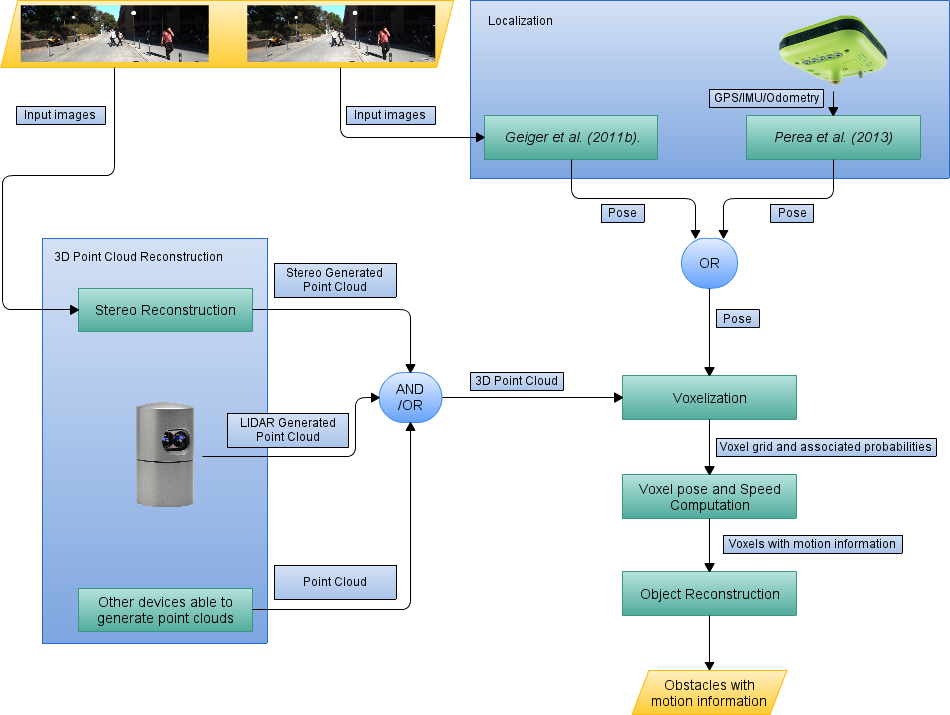
\includegraphics{pipeline_general}
  \caption{Pipeline of the different steps of the method. \todo{Me olvidé de poner el módulo encargado de filtrar los puntos antes de la fase de voxelizado} }
\end{figure}

In the following sections, all these steps will be explained in a bigger detail.

\subsection{3D point cloud generation}\label{ch:chapter05_01_01}

In this stage, a pair of calibrated images is received and transformed into a disparity map, that will allow us to get the corresponding 3D point cloud. In \todoref{XXX}, we evaluated a set of algorithms, including some pre- and post-processing filters, in order to know which of these is the most suitable for outdoor autonomous navigation applications. From this evaluation, we concluded that best results were given by the configuration we named as \emph{Census-SGM Conf 2}. Unfortunately, we had not access to the optimized version of this configuration at the moment of developing the method explained in this chapter. In the other hand, in the same comparison, we saw that both \emph{BT-SGM} and \emph{ELAS} algorithms had also a good response, and we had an implementation of both of them. The question is: what is the most suitable algorithm for our approach? 

If we look again to the charts in section \todoref{fig:cp05_tfs}, we can notice that the response is similar for both algorithms in the chart at \todoref{XXX-LGT,density,alg}, where the density of all the algorithms is compared for the \acs{LGT} based evaluation. The same happens in the \todoref{XXX-alg,NCC}, despite we concluded that the reliability on this measure is still not clear. In chart \todoref{XXX-alg,NFC} the difference between both algorithms starts becoming bigger, with better results for the \emph{BT-SGM} approach if compared to the \emph{ELAS}. Anyway, results for this last method are not so bad, which is quite better if we attend to the average error computed using the \acs{LGT} (See chart at figure \todoref{XXX,LGT,avg}). This last measure is quite decisive, as too much noise can fake the results. If we look at figure \todoref{XXX-comparacionPointCloudELASvsBTSGM} at section \todoref{XXX-polargridresults}, it is possible to see that the noise generated by \emph{BT-SGM} is much more than that by \emph{ELAS}. This is due to the triangulation-based reconstruction of the disparity map.

Finally, if we look at figure \todoref{XXX-comparacionTiemposELASvsBTSGM} in section \todoref{XXX-polargridresults}, we can see that \emph{ELAS} is much faster than \emph{BT-SGM}, and we require a fast algorithm in order to complete the whole pipeline in real time. \emph{ELAS} is able to work at an average of $17\,Hz$, while \emph{BT-SGM} average is below $5\,Hz$ in the implementation used. Considering this with the fact that the difference between them when looking to other measurements is not so big, we chose to use the \emph{ELAS} algorithm as the base for the point cloud reconstruction.

In figure \ref{fig:cp05_tfs}, we can observe the relation between the point cloud generated and the coordinates frame located in the center of the left camera. In this coordinate system, $X$ axis is pointing to the right, $Y$ is the depth of the scene, and $Z$ the height. The rest of frames are explained in more detail in section \todoref{XXX}.

\subsubsection{Point cloud filtering}\label{ch:chapter05_01_01_01}

Once we have obtained the point cloud, we segment the salient volumes by assuming a flat ground. We remove the points below a plane defined by $XY$, as well as those points that are too far from the origin centered at the left camera to fall inside the voxel grid. This distance is controlled by the resolution parameters and the size of the grid, so

\comment{No estoy muy seguro de que esta ecuación sea necesaria ni de que sea la forma adecuada de expresarla}
\begin{equation}\label{eq:cp05_filter_limits}
\begin{cases}
interval_x = [-(grid.size_x / 2) * resolution_x, (grid.size_x / 2) * resolution_x ], \\
interval_y = [0, grid.size_y * resolution_y ], \\
interval_z = [0, grid.size_z * resolution_z ]
\end{cases}
\end{equation}

, where, at each dimension $i \in (X,Y,Z)$, $interval_i$ is the interval in meters, $grid.size_i$ is the size of the grid and $resolution_i$ is the resolution of the voxel.

\begin{figure*}[t]
        \centering
        \begin{subfigure}[b]{0.475\textwidth}
                \centering
                \caption{Full Point Cloud}
                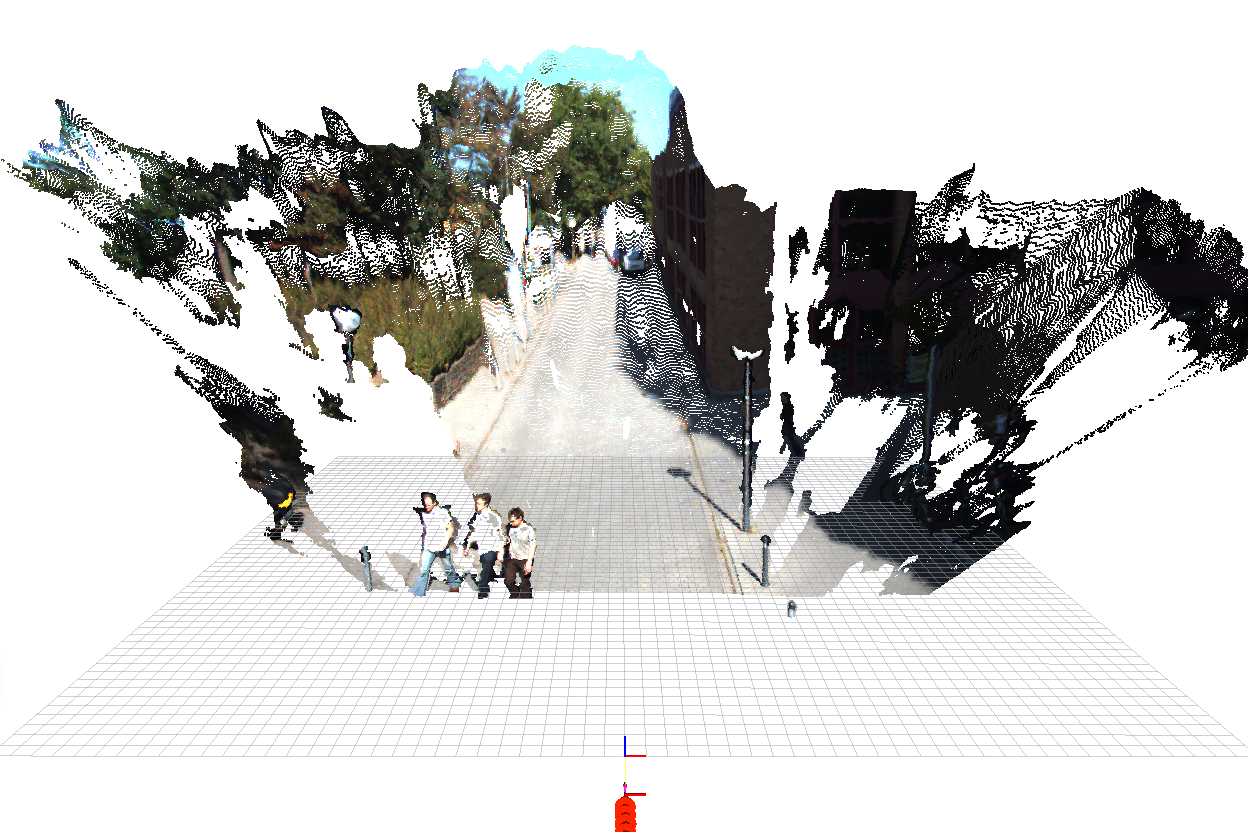
\includegraphics[width=\textwidth]{fullPointCloud}
                \label{fig:cluster1}
        \end{subfigure}%        
        ~ %add desired spacing between images, e. g. ~, \quad, \qquad etc.
          %(or a blank line to force the subfigure onto a new line)
        \begin{subfigure}[b]{0.475\textwidth}
                \centering
                \caption{Filtered Point Cloud}
                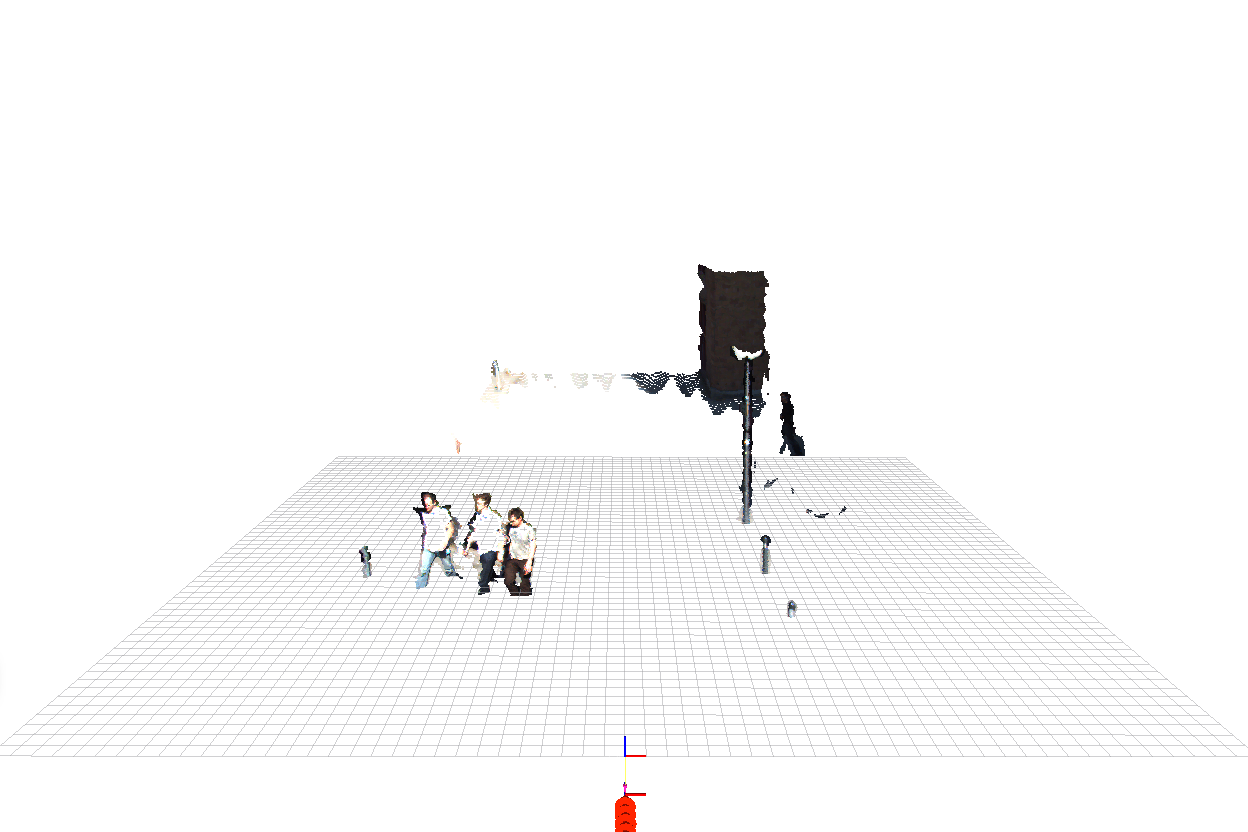
\includegraphics[width=\textwidth]{filteredPointCloud}
                \label{fig:cluster2}
        \end{subfigure}%
        \caption{Comparison of a point cloud obtained using \emph{ELAS}, before and after the filtering.}\label{fig:clusterization_output}
\end{figure*}

\subsubsection{Using other sensors}\label{ch:chapter05_01_01_02}

Despite we have oriented this work to the usage of a stereo camera as input device, the point cloud generation step and filter step have been implemented as separate processes and, as we will see later, no color information is used. So other sources providing a 3D point cloud stream are acceptable for our algorithm. Also several sensors can provide data simultaneously.

\subsection{Ego-motion}\label{ch:chapter05_01_02}

By using a point cloud referred to the left camera (or a given sensor), speeds and orientations are biased by the movement performed by the ego-vehicle between frames. This movement must be compensated, so we need to know the ego-motion performed by the vehicle. This can be done, in one hand, using the localization method used by Verdino (\cite{Perea2013mcl}), based on the information obtained from an odometric sensor, which combined with the \acf{GPS} signal and an \acf{IMU} device, gives a precise localization Other way to do this is by using a visual odometry system, like that proposed by \cite{geiger2011stereoscan}. \notsure{In section \todoref{XXX}, a comparison of a sensor-based odometric system and a image-based odometry system is performed, concluding that \todo{...} }. As some datasets does not include this odometry information, we have decided to use the visual odometry method in our evaluation tests.

In figure \ref{fig:cp05_tfs}, we can see the different positions at which the vehicle has been located at previous frames, as well as the rest of intermediate coordinate frames used in the application.

\begin{figure}[thb]\label{fig:cp05_tfs}
  \centering
  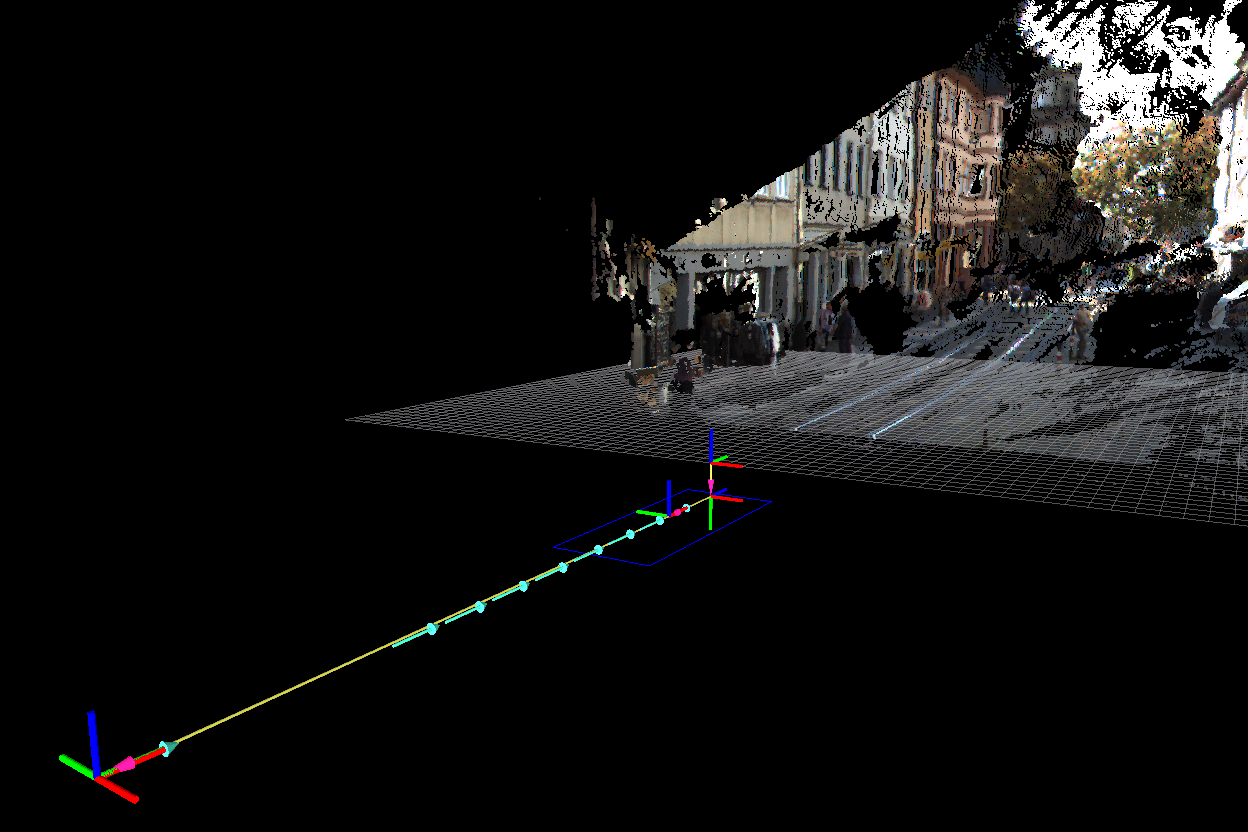
\includegraphics{tfs}
  \caption{Transformations tree used in our application. \todo{Añadir esquema con los frames arriba a la izquierda de la imagen} }
\end{figure}

\subsection{Voxelization}\label{ch:chapter05_01_03}

With the point cloud received from

% Recibimos nube de puntos como entrada
% Cada punto irá asignado a el voxel correspondiente usando la expresión...
% Asignacion de probabilidades (en una subseccion)
% Cada uno de los voxel contiene además información relativa a:
%   puntos 3d asociados
%   sigma en cada una de las dimensiones
%   occupiedProb
%   occupiedPosteriorProb
%   density (numero de puntos3d)
%   vx, vy, vz
%   partículas asociadas
%   obstáculo al que pertenece
% En la imagen XXX podemos ver el resultado de esta etapa, donde cada voxel está representado mediante un color diferente
  
\subsection{Voxel pose and speed computation}\label{ch:chapter05_01_04}

% El pipeline de esta etapa está representado en la figura XXX. A continuación se describe cada una de las etapas:

% Predicción
% ==========
% 
% 
% 
% Measurement Based Update
% ========================
% 
% 
% 
% 
% Inicialización
% ==============
% Sigue un proceso similar al de la fase de inicialización realizado por danescu2012particle, sólo que en este caso empleando las 3 dimensiones
% Poner como algoritmo:
% Si la probabilidad de ocupación de uno de los voxels es mayor que un umbral dado y no hay ninguna partícula en la celda, 
%   inicializamos Nc partículas 
%   
% Nc es el número máximo de partículas permitido
% 
% Cada partícula es inicializada con una pose (x,y,z) = al centroide del voxel, y una velocidad (vx, vy, vz) aleatoria entre 0 y una velocidad máxima pasada por parámetros para cada una de las dimensiones. 
% Como estamos incluyendo la posibilidad de incluir velocidad en el eje z, incluimos la posibilidad de realizar movimientos no necesariamente horizontales. Si queremos limitar el tracking a esta situación, basta con poner el parámetro asociado con la dimensión Z a 0

\subsection{Object reconstruction}\label{ch:chapter05_01_05}

% Segmentación
% ============
% 
% Filtrado
% ========
% 
% Aggregation
% ===========

\subsection{Planning and obstacle avoidance}\label{ch:chapter05_01_06}



% RESULTADOS:
% Imagen que compara los resultados con ELAS y con BT-SGM
% Gráfica de tiempos
% Decir los tiempos en Hz (ya se dijo arriba, pero se puede repetir)
% Añadir comparativa entre libviso y la odometría real
 